\documentclass[a4paper, 12pt, oneside, english, twocolumn]{article}
\usepackage[nf]{coelacanth}
\usepackage[T1]{fontenc}
\usepackage{csquotes}
\usepackage{booktabs}
\usepackage{url}
\setlength{\emergencystretch}{15pt}
\usepackage[dvipsnames]{xcolor}
\usepackage{eso-pic,graphicx}
\graphicspath{ {./ } }
\usepackage[figurename=]{caption}
\usepackage[top=50mm, bottom=50mm, outer=40mm, inner=40mm]{geometry}
\setlength{\columnsep}{90pt}
\usepackage{sectsty}
\usepackage{tocloft}

\allsectionsfont{\bfseries}
\sectionfont{\bfseries}
\subsectionfont{\bfseries}
\subsubsectionfont{\bfseries}

% change color of text, example replace all \color{Goldenrod} with \color{lightgray}
\definecolor{myColor}{RGB}{0, 86, 63}

\color{Black}

\usepackage{fancyhdr}
\usepackage{amssymb}
\usepackage{array}
\usepackage{imakeidx}
\usepackage{microtype}
\usepackage{textalpha}
\usepackage{wasysym}
\makeindex[columns=2, title=Alphabetical Index, intoc]
\linespread{1.5}

\begin{document}
\bfseries
\fancypagestyle{plain}{%
\fancyhf{} % clear all header and footer fields
\fancyfoot[C]{\bfseries\thepage} % except the center
\renewcommand{\headrulewidth}{0pt}
\renewcommand{\footrulewidth}{0pt}
}
\pagestyle{plain}
\AddToShipoutPictureBG{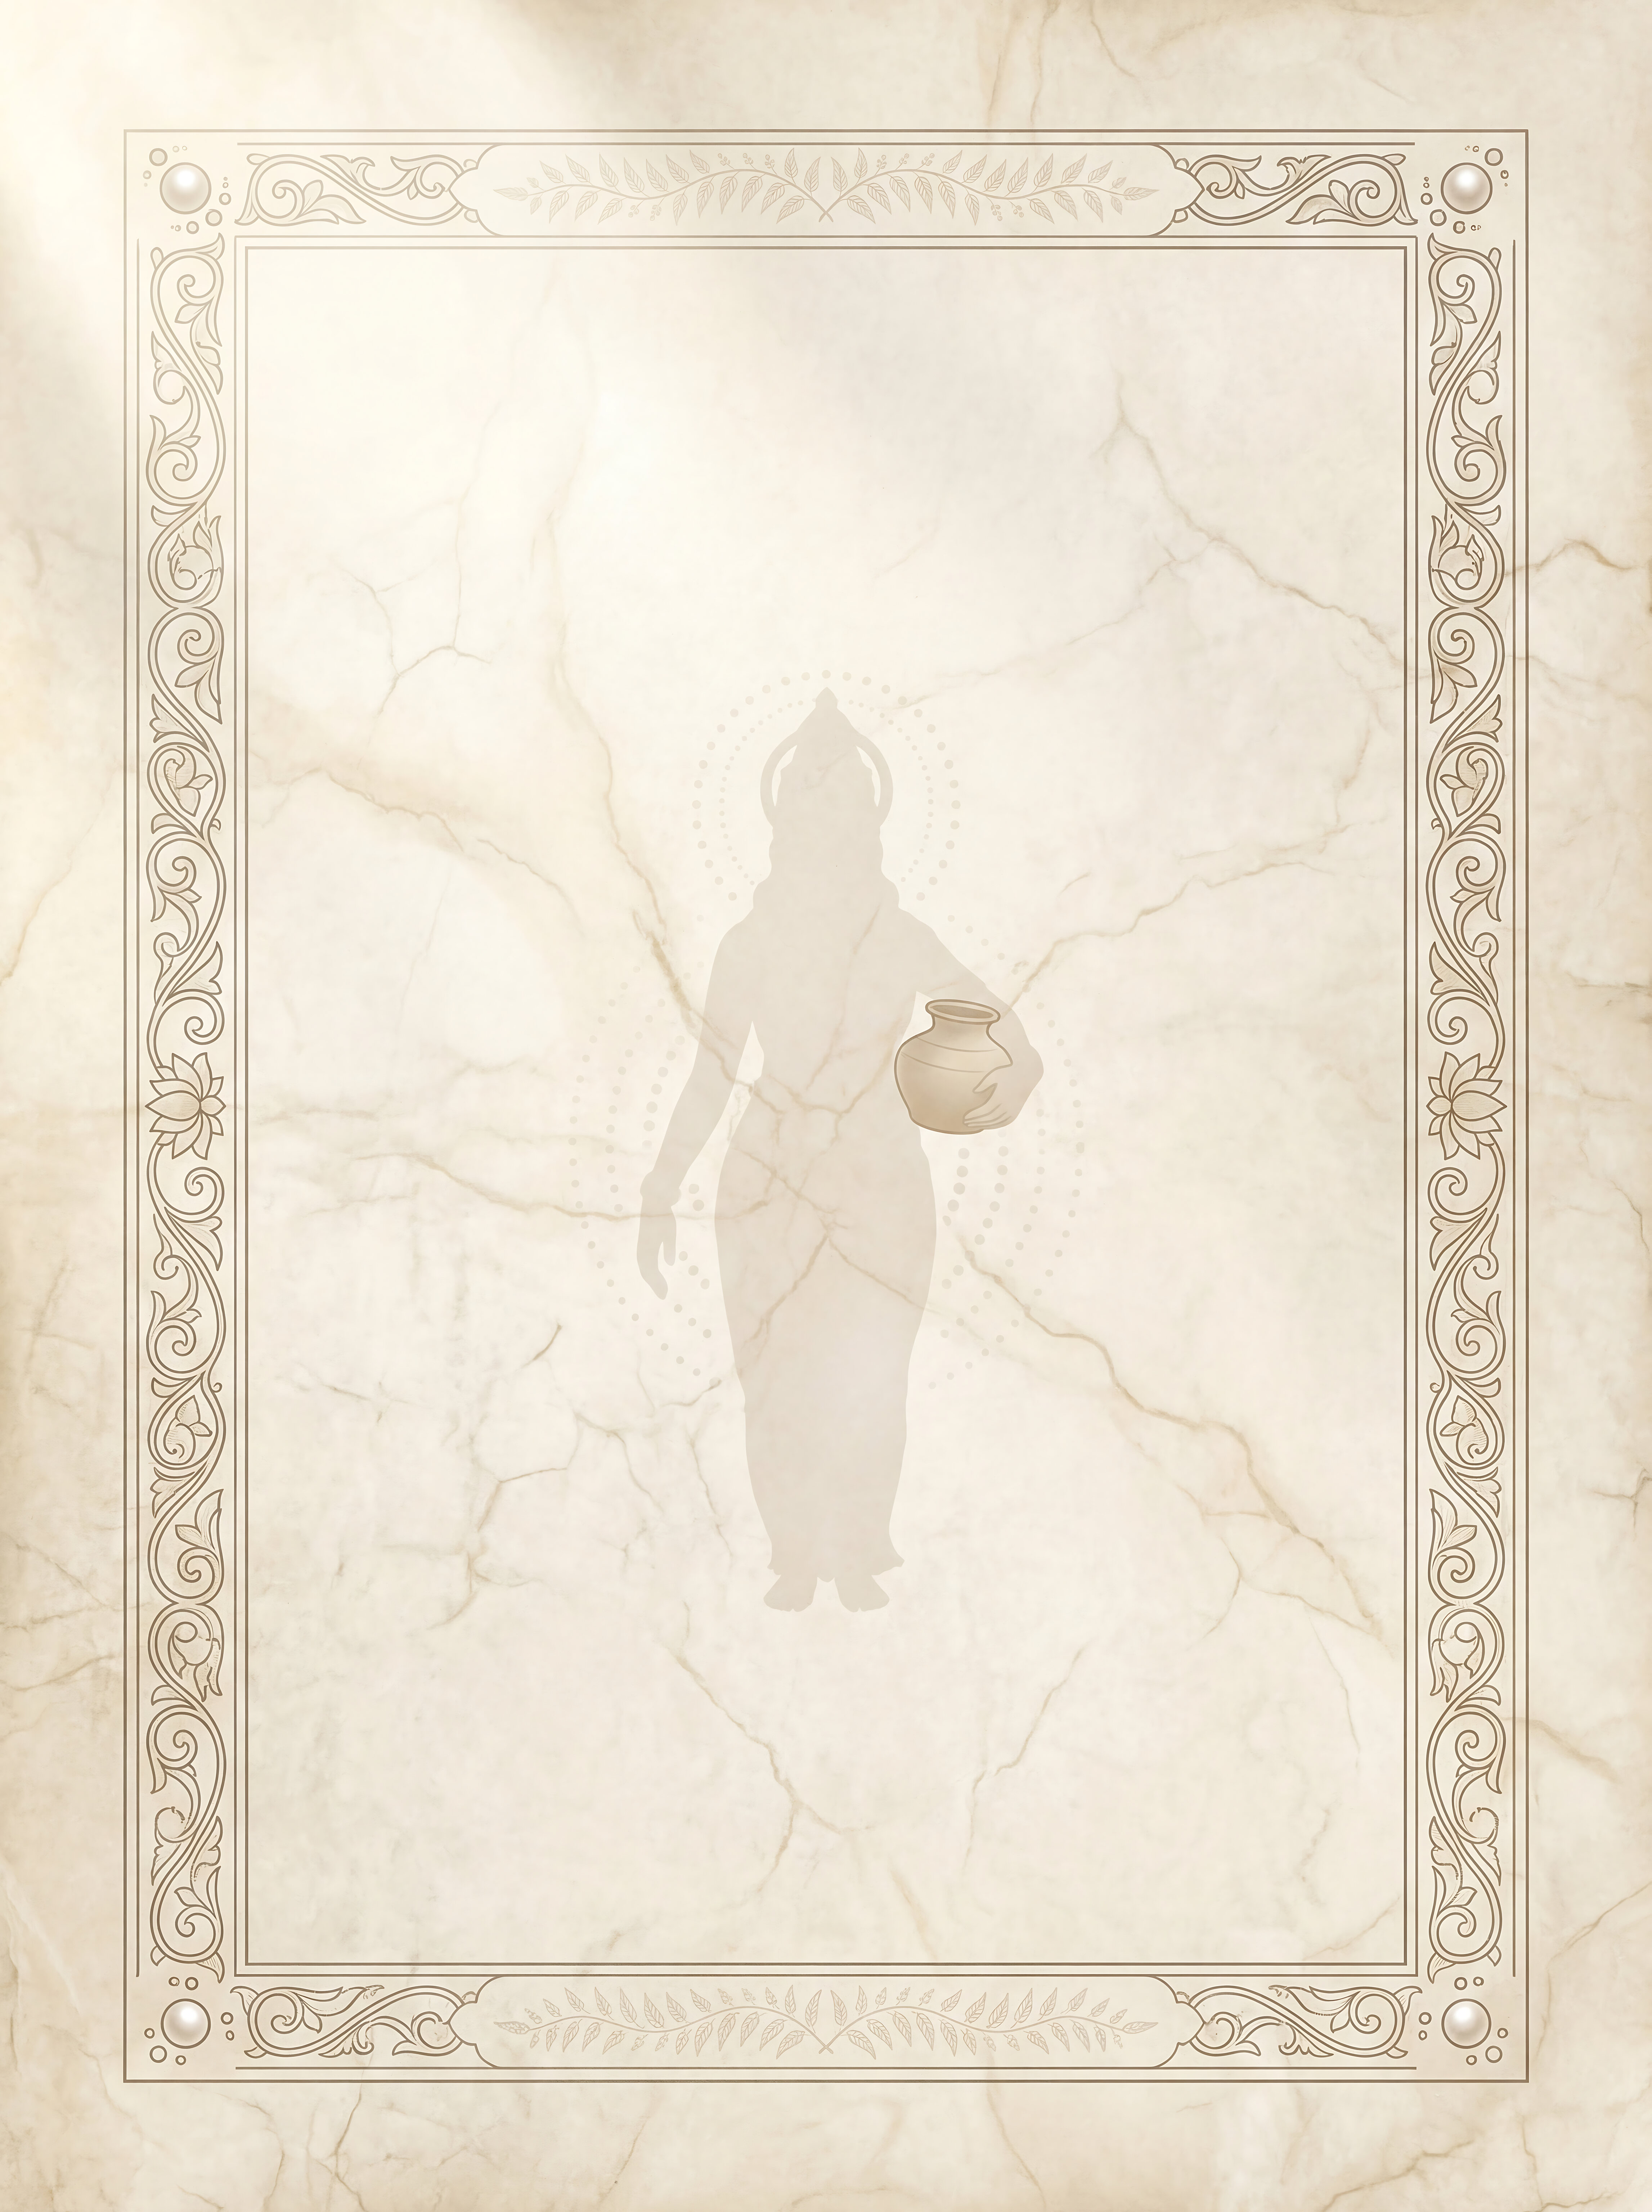
\includegraphics[width=\paperwidth,height=\paperheight]{mariamman3.jpg}}
\begin{titlepage} % Suppresses headers and footers on the title page
	\centering % Centre everything on the title page
	\scshape % Use small caps for all text on the title page

	%------------------------------------------------
	%	Title
	%------------------------------------------------
	
	\rule{\textwidth}{1.6pt}\vspace*{-\baselineskip}\vspace*{2pt} % Thick horizontal rule
	\rule{\textwidth}{0.4pt} % Thin horizontal rule
	
	\vspace{0.75\baselineskip} % Whitespace above the title
	
	{\Huge The Smallpox Goddess} % Title
	
	\vspace{0.75\baselineskip} % Whitespace below the title
	
	\rule{\textwidth}{0.4pt}\vspace*{-\baselineskip}\vspace{3.2pt} % Thin horizontal rule
	\rule{\textwidth}{1.6pt} % Thick horizontal rule
	
	\vspace{1\baselineskip} % Whitespace after the title block
	
	%------------------------------------------------
	%	Subtitle
	%------------------------------------------------
		
	\vspace*{1\baselineskip} % Whitespace under the subtitle
	
	%------------------------------------------------
	%	Editor(s)
	%------------------------------------------------

        {By \large V. V. Ramanan}
 
	\vspace*{\fill} % Whitespace before the editors

        

    %------------------------------------------------
	%	Cover photo
	%------------------------------------------------
	
	%\includegraphics[scale=1]{cover}
	
	%------------------------------------------------
	%	Publisher
	%------------------------------------------------

        {Article from \emph{Siddhanta Deepika}. Vols. 4-5}
        
	\vspace*{0.5\baselineskip} % Whitespace under the subtitle
	
	Madras, 1897 % Publication year
	
	\vspace{0.5\baselineskip} % Whitespace under the publisher logo

    {\small Solar Anamnesis Edition} % Publication year
	
	{\small CC0 1.0 Universal } % Publisher
\end{titlepage}
\setlength{\parskip}{1mm plus1mm minus1mm}
\setcounter{tocdepth}{3}
\setcounter{secnumdepth}{3}
\clearpage
\small
\paragraph{}
It is a thousand pities that the South Indian demonology, spite the work of the ``\emph{Indian Antiquary}'' for the last two decades and more in unearthing Indian folklore, nursery stories and old wife's anecdotes, remains yet a dark problem. Of recent years, we had an interesting book from the pen of a veteran Anglo-Indian on ``Vikram and the Vampire'' narrating the adventures of the celebrated Indian Arthur and those of the Indian Dragon. But a systematic book cataloguing the deeds of all the South Indian Devils, both wild and domesticated, giving diagnostic hints for their respective identification, and a tabulated classification of all their genera and species has long been a desideratum. To name an instance, we have the family of \emph{Kâlîs}, embracing hosts of species such as \emph{Mâri}, \emph{Mahâ-mâri}, \emph{Kâli}, \emph{Bhadra-Kâli}, \emph{Mahâ-mâyi} and the rest. Among the \emph{Pidari} family, we get the \emph{S'ûla-pidâri}, \emph{S'ulukku-pidari} and a whole lot of other \emph{Ammans}. The tame varieties among these are reared in some families as tutelary Devils, which are satisfied with a few chops of meat at a time like the fox-terrier. While, the semi-domesticated breeds like \emph{Pêchi} [\emph{Periyāchī}], \emph{Mâdan} and \emph{Kutti-châtân}, have a preference for warm gore and are often difficult of propitiation. To satisfy them, some gruesome slaughters are now and then resorted to, and the mauled carcases are said to be literally sucked for their blood by these gaseous mammals unseen by man. Thus, they can be made tractable for a time, when the Hindu ought to take care to make use of their invulnerable powers in ruining his inimical brethren. After a time, these grow restive again, and then, unless the necromancer gives his infernal retinue the needful sanguinary fodder, they might ``turn again and rend him.'' As a penalty for his negligence, the Devil-fancier, so far from being left alone with loss of services, is served in turn so well that he would need no more their services, nay any services at the hands of the land of the living. Such is said to be the summary and rough-and-ready nature of their crossed companionship. Withal, man takes care to see that they flounder only in the stagnant limbo of semi-domestication, as a reversion to their original wild state opens him to the danger of their making a meal of him in an instant without any warning. In many cases, therefore, their domestication is not so much to profit himself actively from their friendship as to ward off any wanton rowdyism from them. So to speak, the Hindu has to maintain the companionship of the Devil to keep up appearances. But, the purely wild Devils have enjoyed a free-and-easy life from times immemorial, and the Indian has never attempted to domesticate them, though, in a few instances, he has tried to enlist their sympathy in the hidden infernal hierarchy that is supposed to rule over the welfare and interest of every Indian village and town. \emph{Vîran and Karuppan} with all their species and sub-species belong to this division and they await with vulpine thirst the periodic carnage of animals gracing their animal festivals. These guard the village at nights against evil influences, and avert any pestilential diseases that might frequently be visiting it. In fact, these are the Sanitary Inspectors appointed by the Kingdom of the Devil to look after villages, only their pay is met from the pockets of the villagers instead of the infernal exchequer, and the arrangement reminds one of the system under which the British Government sends its officers to the Native States in times of need. And one of these rural demons is our old friend \emph{Kâli}, the well-known Smallpox Goddess of the English Missionary parlance in India.

The Smallpox Goddess is one of the most mischievous fiendesses that ornament the \emph{Saiva-Siddhânta} Pantheon. Viewed from one standpoint she appears to be the consort of the ferocious \emph{Siva}, rivalling him in her terrific mien, and her feline strength and cunning. In another aspect she appears as an incarnation of feminine immodesty, endued with all the one-breasted valour of the Dabhomi Soldieress, and crowned with a dishevelled hair, the colour of which takes after the dun indescribable fulvous smoke of the washings of a painter's palette. She has jaws always well displayed in which it is easy to descry all the dental perfection of \emph{Felis leo}. Torn entrails of rats and dogs hang from her mouth dribbling blood, while the skirts of her petticoat stand above the line of decency, and this lovely old amazon according to one set of old wife's folklore, is genetically no better than a Pariah damsel. She is said to stalk the streets in still nights with an earthen vessel, in the epidemic seasons, containing in innumerable numbers ``the mystic pearl without price'' --- the Smallpox ``pearl.'' The Hindu fervently believes that the pustules which appear at the close of the preliminary pyrexial symptoms on the body of the patient are only the ``pearls'' which the grim dame strews on his body out of her vessel. When the Smallpox rages in a village in unabated vigour, the mealy-mouthed Hindu has to speak in the so-called Mâri-amman \emph{patois}, if he is necessitated to make any allusion in his ordinary talk to the filthy contagion. He speaks of the benevolent Mâri ``playing'' with her ``fondlings'' should he chance to mention to a friend of his the ruthless devastation going on in the village in the shape of deaths of the patients after protracted sufferings of a malignant type. Even the very patient who is the victim of the exquisite complaint is addressed in one of the many names of the Goddess. Relations near and remote who might happen to visit the sufferer call him as ``Mari!'', and tell him ``don't be angry!'', when they wish to commiserate him for the infinite pains he labours under. The idea is that for the time being the entity of the patient has becomes \emph{nil} and he is filled with the \emph{efflatus} of the ``Mari.'' In fact, he is nothing if not the Mâri herself.

And before we attempt a picture of the religio-medical treatment the patient undergoes after the inmates of his house have once made out unerringly that the disease is a distinct case of Smallpox, it would be interesting to see how the origin of the glorious \emph{Mâri-amman} is accounted for by Indian folklore and mythology.

Parasurâma, the celebrated Indian mythical Hercules, deft at felling human heads by means of his superior axe that could beat hollow in point of massiveness and destructive mechanism even the tomahawks of the American Indians, had a wonderful father and mother. The father was an exemplar of what cruelty and wild disposition can be, and he grew one day angry with his wife. He was minded to take the law into his own hands, as befitting a man-demon of his overflowing animal spirits and to inflict capital punishment upon his wife. But he shuddered doing the act himself, and wanted therefore to make a cat's-paw of his son's assistance in the matter. All the sons of his, save Parasurama, refused to indulge the deed. The homicide therefore fell to Parasurama's share, and he despatched his mother unflinchingly to the other world at one stroke of his flashing axe. The joy of the diabolic father, rich in boons, knew no bounds, and as a reward for the instantaneous matricide, the father asked his son to demand from him anything he liked. ``Restore my mother to her life!'' was the ready reply of the dutiful son. ``Join the head on to the body, and you will see her rising as if from a dream'' was the father's compassionate gift. And now, lo! the head could not be seen. Really some feathered biped or a beast of prey had bolted away with the severed head. What should be done at this crucial juncture? Parasurama stared round and round, walked about hither and thither till at last he picked up in a few minutes a head that he found in the vicinity: but the head was evidently that of a Pariah woodwoman. In his eagerness to see at least the body of his mother vitalised, he joined the Pariah head on to the Brâhman trunk, and in an instant the soldered frame quivered with rising animation, and both the father and the son saw the fruit of their wonderful operation, surpassing all the surgical triumphs of the Nineteenth and Twentieth centuries, the operation of \emph{cephalo-plasty}. This ethnical combination derived from human grafts, this admixture of the Aryan and the Turanian or the Dravidian bloods by processes indisputably superior to those of the present-day Aveling's Transfusion Apparatuses, is our old friend Mâri. What this myth denotes, what historical facts underlie the surface stories, whether the Mâri-amman's genesis is only another name for any ancient social upheavals, are all outside the range of our present discussion. In any case, the improbability of the tale is only too patent, and it is certain the Goddess and all her associated stories of extreme marvel are consummate concoctions improvised, to account for a disease that has been plaguing India through all times. Since it is in the nature of the Hindu himself to account for every phenomenon he is cognisant of, in terms of the doings of his old-world mythical demons, and to bottle each superstition with theological labels and put it in the laboratory of his nursery tales and ancestral tradition, we need not be fretting our minds here as to the why and wherefore of the present fable.

This, the necessary digression relating to the genesis of \emph{Mâriamman} over, we can now see how the religio-medical treatment is conducted when a patient has fallen ill of pox. Prior to the visible manifestation of the contagion, the would-be patient suffers from a feeling of dull languor and mopish break-down. He does not relish food properly nor does sleep give to his body the required amount of rest and peace. Slowly a fever invades him subjecting him to terrible fits of vomiting. The temperature of the body rises from hour to hour, till at the close of the fever, his head swims and he is invariably in a delirium. In the case of certain patients, the delirium proves itself an unmitigated bane, and the ``exoteric'' signs of their ``astral experience'' will provide wonders even to a special student of mental aberrations. The patient talks gibberish, sometimes a diglot, at other times a triglot, nay, even a polyglot mongrel, made up of unintelligible language and inarticulate sounds, the whole affair enormously terror-striking. Now and then, he starts up from bed with the blood-shot eyes of an inebriate, walks violently about the house, swooning down eventually on some spot, unable to bear the fatigue of his own boisterous exertions. This is the stage of great anxiety to the inmates of the house. After a time, the body of the patient becomes suddenly covered with a crowd of rosy patches which after the subsidence of the fever and the delirium, resolve and develop into pointed eruptions, finally to become the characteristic smallpox pustules. During the pyrexial paroxysms, the patient is believed to be on the eve of the privileged entry into the portals of \emph{Mariamman's} citadel, as the ticket for admission has already been issued to him. He is practically enjoying at the portico the sight of the inestimable doings of Her Supreme Diabolic Majesty's militia. Thus the bed-ridden wretch is for the time being under the jurisdiction and governance of \emph{Pêchi-A'yi} the head-portress and staff-bearer of \emph{Mâri}.

Here we may pause to note how \emph{Pêchi} looks, and what role she plays in spreading the contagion. She is the chosen commandant in the infernal army of hobgoblins, salamanders and undines that are said to tread on \emph{Mâri's} heel, and hence the right finger of the Smallpox Goddess. Her face reminds one of that of the Royal Bengal Tiger as it stands surveying all around with a threatening mien, ready to pounce upon any intruder, while at its feet lies the newly-mauled deer, suitable for a rich meal. She puts on a tucker, which only assists to set her formidable-looking pendulous breasts off to greater effect. She is not a young dame by any means, but a blood-curdling shrewish old hag, with the bones of her battered body prominently showing out, and the coriaceous elephantine skin pinched and shrivelled up, ever on the look-out to dart at any healthy individual, and to lash into his system a great amount of smallpox virus. And nearly nude is she in her narrow strip of cloth round the waist, and with matted and dishevelled hair, and grinning teeth, like Death incarnate, she dances her demoniac dances to the resonant roarings of the hobgoblin bands. It is said that the patient's frightful groans, shrieks and frequent startings from bed to run about in maddened fury, are all occasioned by the fear he perceives from seeing the frantic merry-making and the deafening pandemoniac howls of the hellish brigade.

And naturally enough, the inmates try to do anything and everything in their power according to their lights to alleviate at the present crisis the patient's suffering by making the prescribed offerings to \emph{Pechi}. She is fond of loaves of the pattern of the Jewish \emph{show-bread}, made of the flour-compound of four different kinds of grain, and of some slices of coconut kernel, but without salt. So long as the delirium lasts, the offerings are prepared assiduously every evening, and thrown off on the roof of the house with a pity-evoking call upon \emph{Pechi}, to take them away and relieve the sufferer of his soul-tormenting fears. If for all the propitiatory fodder to \emph{Pechi}, the patient in his delirious walkings and violences be beyond measure uncontrollable, and if there should be any possibility of his getting away unawares from the house, during his raging state of unconsciousness, all the doors of the house are well shut and bolted making any attempted exodus after the enforcing \emph{Pechi} impossible. For, it is said by age-worn matrons that, should at this stage he make an exit and \emph{people in the street gaze upon him}, \emph{Mâri} would get trebly ferocious and do away with him altogether.

In a few days the delirious condition cools down, the eruptions become more and more visible and the patient feels day after day the increasing pain all over the body owing to the intense and continuously rising inflammation. Having by this time thoroughly regained his consciousness he smarts under the agonies that prey upon him. The vesicles have grown larger and bigger and the skin has become tense and painful around them. In some cases they may be so thick-set as to leave no room even for a pin-prick. Now and then the miserable sufferer is in a stupor through excess of burning pain. He howls and whines, and often even roars with unutterable rage and despair. To lie on his back would be a difficulty for him, for, all over that region there are enormous pustules. For a similar reason, he cannot repose on his sides, nor on his face. Neither can he sit or squat, nor even stand on his legs. The sole of the foot, the scalp, the interior of the nose and even the white of the eyes are invaded by a multitude of excruciating eruptions. Again, when the pustules have advanced in development, an unbearable itching sensation is felt at every point on the body, in addition to the previous pain and the feeling of burning. Even the most downy quilt will be nothing short of a prickly bed of thorns. The only commiseration for all this he can legitimately expect from his friends and relations, is an address to him now and again as, ``\emph{Maham-m-mâyi!} Please don't fret. \emph{Maham-m-mâyi!} Please don't be angry. I beseech you not to trouble the child, I shall present you with an offering of a couple of mud eyes, and I shall give you a cooling, refreshing bath of tender coconut water.'' They mean by such prayers that they will do all in their might to appease the Smallpox Goddess, that she may deign to let the patient alone, without much hurt.

As soon as the state of delirium has passed, and small pinkish vesicles have made their appearance on the body, the inmates of the house get hold of some of the oldest --- nearly always widowed --- crones in the village, to diagnose the case properly. These old gossips are credited with a greater experience of eruptive affections like smallpox than even the best European dermatologist, and unless they certify that it is a distinct case of smallpox, the people in the house may not begin the necessary medico-religious observances enjoined by tradition in the case of smallpox, and smallpox alone. And so the old women with their shrivelled-up skin, toothless mouth and white-hooded face, who are a hideous spectacle by themselves, crowd round the bed-stead of the patient in the early morning, remove the sheets off his body, and start an inspection of the eruptions on it. Meantime the patient is crying aloud unable to endure the agonies, and after deep deliberation the women unanimously pass the verdict, ``It is a case of Maha-Mâyi. She has strewn her pearls richly. Put up a `Pot' in a separate room and invite her.''

The ceremonial of praying to Mâri to come to an appointed room of the house, and of inducing her, by entreaties to linger there till the inmates give her submissive leave to repair elsewhere, is very interesting.

A battered and bruised big brass-pot, of antediluvian appearance, the outcome of indigenous industry, is chosen, and filled with water it is left in a room that may be temporarily set apart in order to invoke \emph{Mâriamman} for consultation and advice on various points in connection with her specialty. The mouth of the pot is plugged with a bunch of margosa leaves which, in turn, is surmounted by a husked coconut with the ``Kudumi'' not torn off. The ground immediately in front of the sacred pot is converted into an altar for \emph{Mâri}, on which will be found displayed to view, all the various things supposed to be her pet food. We can expect to find a handful of a peculiar preparation of roasted rice, known in Tamil as ``Aval,'' a bottle of coconut-toddy, some cigars, and a few young coconuts of big size with a portion of the greenish rind chipped off. For, we must remember that whatever may be her savage or barbaric look, in point of smoking or drinking she is inferior to no fashionable of this dawn of the Twentieth Century. She is not a member of any ``Temperance Association'' or ``Temperance League,'' and teetotallers in her opinion are a set of inane noodles. We may also find on the altar, a large quantity of `cold rice' soaked in a liquid that is in an advanced stage of fermentation. The most aged woman available in the house takes charge of the room and its contents, and the various ceremonies she has to perform as \emph{Mâri's} officiating priestess \emph{pro tempore}. Every morning all the old offerings are removed and new ones are put in their place; the former are given away to Sûdra menials and to Brâhmin boys that may chance to visit the house. Here, before detailing the way in which the old offerings are doled out, we must pause to note an important fact which accounts for more smallpox patients among Hindus than among Europeans.

The European nations avoid the contagion by dreading and fleeing from it, while the Hindu courts it from the superstitious fear that he provokes the wrath of `Mâri' in case he does not willingly place himself under her `merciful sway,' when there is an opportunity. The smallpox may be raging in a village and may be carrying off men and women as victims in large numbers, yet the Hindu will hardly dare to hear any advice coming from a sanitary or vaccination inspector as to the ready means of keeping it in check. Instances are not uncommon when a vaccination inspector visits a village with his `lymph' and `lancet,' while the Brâhmans try to send him away with bribes. They do not want the Englishmen's `false-pearls,' for to see counterfeit things smuggled into her port will excite \emph{Mâri} to greater anger and she may `play away' then with the population only too heartily. Such is the belief of the orthodox villager towards vaccination.

Now to go back to the skinny, ugly `priestess.' She rises quite early in the morning, goes to a tank in the vicinity, bathes and returns home with a narrow-necked brass-pot filled with the tank-water. As she is coming, she may not even touch or speak to others, such is the sanctimony that attaches to her clothes, soaked through and through with water, and clings to her weather-worn pinched-up constitution, when once she takes upon herself the onerous office of the priestess at \emph{Mâri's} shrine. Nobody could even think of going near her lest the holy air investing her body should get vitiated. As soon as she comes home, she casts off her wet garments and puts on dry clothes that were kept in a lonely spot beyond the polluting reach of any other human being. After wearing her garments, she begins a course of mock-begging at the houses in the street, demanding from their inmates in the name of \emph{Mâri} ``measures of pearl.'' In each house, they present her with `cold rice' in great ceremonial austerity. And her begging bowl which is generally of large capacity is brim-full before she returns to the infected roof from her trip. Then she enters the room of `sanctum' in the house, empties the water that was put the previous day from the brass-pot, and replenishes it with the tank-water newly brought at dawn. Afterwards, all the old offerings on the alter are removed, and new ones are substituted in their place. Thus, the old ``cold-rice'' is taken away and the new ``cold-rice'' eked out by ``begging'' is thrust in its stend. The old coconuts are removed and fresher ones are brought in.

Meantime crowds of children and boys are making their appearance into the infected house at the especial request of their parents that \emph{Mâri} might condescend to come down and ``play.'' These members sit at \emph{Chota-Hazri} in the house, when the old ``cold-rice'' that stood at the altar as an offering is served to them that they may eat the smallpox ``pearls.'' One belief is that each grain of the ``cold-rice'' is a ``pearl'' of \emph{Mâri}, and their consuming the food will be instrumental in bringing about a mild invasion of pox. And the old water of the brass-pot is also dashed on the body of these innocents, as it is thought that it is nothing short of the holy ``purulent matter'' of the smallpox pustule. Some of the younger boys are brought near the bedstead of the patient that they may readily receive ``the grace of \emph{Mâri}.'' Under these conditions it is easily understood how Hindus manage to victimise themselves on Her infernal altar. This self-hurling into the pit of Death is no better than the Moabite habit of burning, rather roasting children alive to appease the grim, blood-thirsty Moloch. The other offerings are dispensed to Sudras saving the unhusked tender coconuts which are used as the main drink of the patient in the hot afternoons. The remnants of the previous day's offering of the gently sour ``cold-rice'' and cold-rice-water are the food upon which he may be chiefly said to subsist.

One thing to remark in this connection is that in the case of smallpox, even though there might be a slow fever present, the patient's regimen contravenes out and out the normal dietary in ordinary cases of fever. In fact, the cold-rice and fruits which are invariably given to the patient would be the last thing to be recommended to him when he is ordinarily afflicted with febrile symptoms. Thus people fear more Mâri's dictates, than even the demands of temporal hygiene.

The pain of the patient increases with the ascent of the sun in the heavens, and the burning and itching are aggravated a good deal in the hot afternoons by the noisome flies which flit about buzzingly on the body of the patient attracted by the foetor exhaled by his suppurating pustules. To allay this itching sensation the ``priestess'' sits by the bed of \emph{Mâri's} ``chosen subject,'' and gently passes again and again a bunch of margosa leaves she holds in her hand over the patient's body. This operation she may be engaged in, night and day. It has the double advantage of driving off the flies and relieving the unbearable itch. A fan of palm-leaf is also used occasionally. But the Neem is the special badge of Mâri's Service and it should be used unceasingly. No English medicines, however effective in doing good at this stage, can be permitted. They will merely say that they are not approved by Mâri's diabolic legislation, and their use may end with the unappeasable wrath of Mâri and the summary penalty of malformation of the limbs, disfigurement of the body, or death. Bananas are commonly given to eat, coconut-water for drinking and ``cold-rice'' as food.

Days elapse in this fashion with the above monotonous in-door ceremonies when the pustules gradually ``blacken'' and ``wither'' from the region of the head downwards. The out-door religious ceremonies at this time have to do with the propitiatory acts at the temple of \emph{Mâriamman} situated amidst the ``Grâma-Devatas'' of the village on the roadside or elsewhere. We have further certain religious rules restricting the sort of men and women that can be admitted into the infected house and governing the method of cooking to be adopted. These we will presently consider \emph{seriatim}.

Readers of Walter Pater may well remember his observations in ``Marius the Epicurean'' on the priesthood of Aesculapius, and the value of dreams thought to be inspired by the God of Medicine, in supplying information about the origin and development of diseases. If among the ancient Romans, dreams were the sole channel for ascertaining the mode of treatment of a particular disease, the symbology of clinical discipline was most effectively mirrored in the look and appurtenances of Aesculapius, the cure of ailments was more religious than medical not less so, have been the ruling Dravidian practices in relation to the treatment of many contagious diseases over which demonalatory holds such unbounded sway: only in place of the Roman dreams, we have put in the Hindu delirious ravings.

We have referred already to the unmeaning gabble, sometimes positively frightful, that proceed from the patient, during the stage of the delirium coming on straightway in the wake of the eruptive fever, in ninety cases out of a hundred. The sufferer lives and moves and has his being in a world of his own, thoroughly oblivious of what is passing on about him, and talks of things which will be palpable perhaps only to a deranged imagination fired with the excitement of a high fever. His incoherent talk interlarded with groans and shrieks, is a Chinese puzzle to his relations that sit hard by, endeavouring to read a meaning out of his flippant words. He is Mâri's oracle, and ought to be listened to with abiding reverence and interest, as every unmeaning syllable of his, might veil some sober truth or premonition, having a direct bearing upon the prognosis of the complaint, and afford a clue to the extent of the spread of the contagion, and the range of mortality from it in the village. Many women who pose, by reason of their past experience, as experts in interpreting oracular effusions, sit near him, and cross him with subtle questions. \emph{Mâri}, they say, speaks through him for the time, and true and trained interpreters could make out her intentions easily. Queries like these are put to him, ``How many houses you propose to visit? Where do you come from? What time you will stop in our place? How many deaths there might be at the village? Then many a time Hamilton's well-worn definition of Metaphysics said to have been given by a farmer with his bland flatness, is borne out to a letter, and everyone becomes an authoritative expounder of mystic and recondite divinations. In a few cases, what looks like a relevant answer will be obtained though it may not have a shadow of truth in it. The meaning one should attach to such show of relevancy gets clear it we know the secret of how to prolong the somniloquism of a dreamer by throwing out ``a suggestion'' as they technically say, or suitable ideas to keep up and develop the train of fancy passing in through dreamer's mind. Similarly, the highly-strung imagination of a disorderly mind, as that of the patient, could be made occasionally to run in the desired groove by repeated clever questionings.

As the patient is groaning under the ill-starved roof, to the dismay and despair of his anxious relations, the good man of the house has already converted the temple of \emph{Mâri} situated on the roadside, or elsewhere in the vicinity, into a scene of the most pious devotion. The gruesome severity of the Goddess is a great deal enhanced by the crumbling exterior and the haunted look of the temple and the sullenness, nay, the appalling nature of the ceremonies conducted there. The temple is not a piece of elaborate architecture or costly masonry, but a simple tile-roofed building, without even the outer court or the imposing, ``Portico,'' if we may use the expression, of the ordinary Hindu Pagoda. The dearth of any vegetation round the temple, the grim colossal idol of \emph{Pechi} at the gate-way, the altar of red brick-work in the open in front, usually breast-high, bearing a large, dark, iron trident that has been bedaubed many a time with the blood of immolated goats and fowls, all these combine to create in the Hindu's mind an awe which rises in intensity with the intensity of devastation in the village, during the reign of the fell epidemic, and which assumes an almost superphysical aspect to the quailing devotee, as he sees the solitary temple in the scorching glare of the cruel Indian summer. At the expense of the infected house, the priest of the temple called \emph{Pujari or Pandâram}, starts a new routine of devotional acts. In the morning, an elaborate \emph{Archana} is made consisting of the offering of flowers of different hues and varied fragrance; camphor and frankincense are burnt, whose fumes filling the temple-house with an unutterable odour of sanctimony and divine grace, known sometimes to \emph{translate} the souls of votaries; and ``holy ashes'' scrupulously prepared by complicated processes of sieving and sifting are offered at the feet of the granitoid image, with the mumbling of incantations. The ashes are brought to the house as a matutinal charm, and they are smeared over the forehead of the patient and sprinkled into his mouth, in order to stave off virulence of the contagion to any bad degree.

At noon, the ground adjoining the temple is carefully watered on all sides by special labourers employed for the purpose that the mind of the Goddess may grow ``cool.'' The idol also is frequently bathed in a mixture of milk, honey and clarified butter. The water of many tender coconuts is used at intervals as an intermediate ablution. Such propitiatory acts relieve the mind of the inmates of the house, a great deal, of the panic of any further suffering or molestation from \emph{Mâri}, since they, it is thought, will tend to lessen the burning sensation and the itch, so incidental to the contagion, in the scorching and sultry afternoons which are a special feature of the Smallpox season in South India.

As the day wanes, and nightfall commences, the round of ceremonies conducted in the morning is again repeated at the temple, and the ``holy'' offering of ashes is sent to the house as ``the precious Gift'' for the use of the patient. The routine of the ``extraordinary'' temple-service will continue, so long as the pustules go on actively developing when the pain is intense and smarting unbearable.

In bad types of smallpox, through the intensity of the invasion, and the multitude of pustules that plague the sufferer, cataract in the eye is brought on now and again, and sometimes even distortion of the body, telling upon the gait and the erect posture. When the inmates entertain the faintest suspicion from symptoms that are already manifest, that such deformities might occur, they pray to the Goddess that they would present her with votive offerings of mud eyes, mud legs and so on, should the deformities be averted. It is such presents, the result of vows, that catch first and foremost the gaze of the beholder, as he is brought face to face, for the first time, with any Mâriamman temple. The accumulated mud-offerings of years, many of which in a rapid state of decay, may be seen crowded together unceremoniously in front of the temple, not to mention the images of men and women of baked mud, standing as so many servitors of the Goddess in hideous array.

Another vow taken in given-up cases of Smallpox is to give ``a dance'' in her honour, which is peculiar, and must be undertaken only by a special set of Sudra men and women, who form professional companies, and who could be engaged for payment. It is only during the time of the annual festival of the Goddess that such a dance ought to be celebrated. As the dance is an institution playing a very important part in the social life of every South Indian village, it will not be out of place here to give a brief account as to how it is conducted, and what the nature and status of the performers are.

The dancing companies are itinerant and make a living by undertaking ``dances'' for people who have taken dance-vows to the Goddess. Men and women, boys and girls, from among the low ranks of the Sudra community contribute to their number, and the women that join such companies are notably of low morals. They combine with their dance a rude mode of opera-like acting, singing snatches of wild ballads, doggerels, and bazaar-lyrics which are in the mouth of every Indian beggar, street organ-grinder, cart-driver, and jutka-wallah, exuberant with much of animal spirits. The inmates have appointed in their vow a particular annual festival of the Goddess to fulfil their promise. The annual festival runs to as much as even a month in some villages, and a day out of it, is chosen for making good the vow. The priest of the temple is given notice of the fact on that day, so that he may arrange to take the idol in procession round the streets in the evening and bring it to the desired house at night. Meanwhile, the manager of a dancing company specially stopping in the village on account of the festival season is sent for, and on the terms being settled is asked to come with his retinue and the requisite furnishings soon after the idol reaches the house, which will generally be at 8 P. M. Before this, a large shed will have already been erected in front of the house in view of the intended reception to the Goddess and the forthcoming dance in her honour.

At one end of the shed, the fully decked wooden image of the Goddess, which is usually varnished with a thick red shiny paint, is seated in great pomp after the procession has been gone through. All the people of the street assemble there and prostrate themselves before the image and indulge in every pious gesticulation. The dance which is invariably conducted in the presence of the image is supposed to be witnessed and enjoyed by the Goddess ``unseen by man.'' Though it is usual to begin the dance as soon as the idol reaches the house, yet, if it is an early hour, they sometimes put it off till it is as late as ten or eleven P. M. By the time the dance will commence, all the people in the street are ready after their supper for the coming recreation, munching their betel-nut, and assembling under the \emph{pandal} with screams and laughter to witness the interesting performance. The clouty population of Sudra menials with their stolid sons and daughters who make up the greater part of the sight-seers on the occasion, grace the assembly not a little.

The pit, the stage, and the firing room are all one and the same. The mud-covered floor under the \emph{pandal} affords enough room for the various functions of the actors and spectators. Nothing is screened off from view as there is hardly any need for the actors to change apparel or trappings. Each actor comes dressed once for all in tawdry native costumes, pleasing to the crowd, with head-gear and the rest made of ordinary wood, coloured varnish, plaster and tinsel. The same might be said of the actresses also who probably put more paint on their face. Any scene, nay any situation is improvised with the readiness and rustic simplicity of the proverbial fairy-acting in ``A Midsummer Night's Dream.''

Now, the sound of the weird bag pipe begins to roll on the air making a mewing music, while the sickening thirds on the tabor keep time and the clamorous cymbals jingle incessantly. Big shallow-bottomed \emph{chatties} filled with oil (not the petroleum by any means!) are fixed on tall posts. Thick wicks knotted and twisted, of the size of one's knuckles are immersed in the oil and lighted. These primitive lamps which are placed two on each side of the ``Boards'' do duty for the costly appliances used in the English dancing-hall.

After the preliminary flourish of ``mewing'' and ``thudding,'' an actor appears on the scene whom the audience is presumed to take for a king of the old Heroic period of the Mahabharat. His queen joins him presently, her face rippling with smiles. Both sing songs and crack jokes. A Prime Minister and a Clown appear by and bye. All these mix together and exhibit to the audience some pantomime, a few attempts at coarse repartees, some snatches of libidinous love songs, a few gallant-like acts. There is deafening vocal music now and then, and ample demonstration of provincial slang in language and manners. In fact the ludicrous attitudes and gestures which actors and actresses put on, the drollery twinkling in their eye, the clownish nature of their behaviour and deportment, the tones, now drolling, now gurgling in which they carry on their conversation, abounding in fantastic quips and jokes, all these beggar description. Thus the hours wear on till it is almost day-break, when the play closes, the actors are paid by the goodman of the house, and the Goddess, after the inmates have taken leave of her in the usual style, by burning camphor and frankincense and ``offering'' betel-nut, repairs to her temple-home on the shoulders of the men who are appointed to carry her.

The above description will give a fair idea of the so-called ``dance-vows'' for \emph{Mari Amman}, taken by the inmates of the house, when they have reason to despair of the life of the patient from any alarming symptoms. But one of the most prominent of the rites that is undertaken in the house during the patient's agonies, as the vesicles are advancing in development is the costly dispensing of rice gruel to the Sudra menials in the village.

A large quantity of rice, even as many as \emph{four or five markals} at times, mixed with \emph{dhol}, pieces of tender coconut kernel, salt and abundant water is boiled down to a very liquid sort of savoury \emph{Kanji} and distributed to numerous Sudra people including young children, on sultry noons. This treat is repeated every second or third day till the pustules ``blacken,'' shrivel and tend to slough. The recipients swallow the gruel with keen zest, soliciting loudly, as they do so, ``the gracious company of the sweet-Goddess,'' \emph{i. e.}, an invasion of smallpox that would be mild and not painful. The \emph{Kanji} being a gift dispensed to honour the presence of the Goddess, it is supposed that those who partake of it will surely have an attack of pox, but never of a fatal or dangerous nature as they voluntarily implore her ``to set her seal'' on them. Though the distribution of \emph{Kanji} is believed to be a means of pacifying \emph{Mari}, the deafening noise the menials make as they crowd at the street-door to partake of the distribution never fails to annoy a good deal the woeful sufferer within. So much so, that during the performance of the \emph{Kanji}-dispensing ceremony, the patient oftentimes imagines it were better he was left alone than subjected to the inflection of such horrid yells from the people at the irritating mid-day.

The restrictions observed in regard to the admission of people into the infected house are varied and must be closely looked into. Enthusiasts possessed of ``Indo-mania'' may try to read the inculcation of the best principles of the most approved modern hygiene under those restrictions. But one who studies the facts with dispassionate judgment and unbiassed reason, will best be able to judge whether hygiene any more then steps to stave off further progress of the contagion, is ever contemplated under the mask of such time-honoured injunctions. Now, what are the actual restrictions obtaining under the infected roof? A pure virgin, a wife, that did not enter into sexual relations with her husband the previous night, a bachelor of unsullied morals, a married man that ``knew'' not his bride within the past 12 hours, and all widowers and widows of no loose character might go into the sick room and visit the patient. One that has had a recent shave or an ``oil-bath,'' a maiden or woman using scented cosmetics or ``painted with saffron'' will never be allowed to reach the bedside of the patient, not one who had just returned from any outstation. Even parents are never permitted to see their child should they chance to come from any outside place, however much they may anxiously yearn. The son will probably have taken pox whilst stopping in a town whither he may have been sent on some purpose by his parents, and they will have come from their home in great flurry on an urgent message, extremely eager to see their darling; yet they could never be allowed entry into the house, immediately after their arrival. They ought to stop elsewhere in the town for a day or two, and after a sufficient lapse of time, ranging from 2 to 5 days according to circumstances may get admission into the infected house. The inmates should be free from all ideas of ``wedded-life'' till the Goddess ``goes out of the house; if they are not, they would quit the house altogether. The entry or retention of people happening to be of different description from the above, is sure, it is thought, to kindle the rage of the imperious and sulky divinity; as a consequence, the patient might suffer enormously from the pangs of the disease, if the Goddess in her anger is so forgiving as not to make away with him. The malformations and the deformities incidental to patients emerging out of a bad attack such as blindness, lameness and other disfiguring distortions and even occasional paralysis are nothing else than punishments inflicted by \emph{Mari} for violating her dictates.

Again, within the house itself no tasteful toilet or gay decoration is permitted. There should not be any loud outburst of laughter, nay, any indication of merriment, and everything ought to be grave-looking without even a shadow of light-heartedness. They are not to hold a sumptuous banquet inviting friends and relations, and are further strictly prohibited from preparing any dish involving frying. The use of sesamum or coconut-oil for culinary purposes is discountenanced, not to mention its service during bath or toilet. Bu in their stead, castor-oil or ghee can be used with perfect immunity. If the patient was married, his bride, should quit the house and live away from it till ``the Goddess left the house.'' Any slight infringement from these rules may result in something dismally injurious to the sufferer.

Tradition has it that the smallpox patient should on no account be allowed to travel, for \emph{Mahamayi} will little brook any default on the part of her conscript in that direction. And mention must also be made of the widespread belief that there could be no worse crime under the Sun, putting an affront upon the Goddess' legislation, than the patient's shifting to his bride's house. The fate of the sufferer will then be almost sealed, and the virulence and magnitude of the attack will pass conception. But, according to some high priests of demonolatry, who might outdo Jesuits in casuistry and hair-splitting explanations the degree of penalty will lesson with individual circumstances of extenuation, Thus, differences are contemplated between the patient who repaired to the residence of his spouse of his own free will, and the patient who was removed to his bride's house without his consciousness or will, by his friends or relations, between the sufferer who was tarrying at his father-in-law's-residence when casually overtaken by the disease, and the sufferer who reached his father-in-law's house after the symptoms were once patent upon his body.

We may presume for the sake of our present account that the patient has not transgressed any of the recognised enactments of \emph{Mari}. At the point we have now reached, the stage of unconscious raving will certainly have passed away. The stage that succeeds it is far worse. Consciousness has become thoroughly restored only to make him doubly alive to the inflammatory pain all over his body. As has been already pointed out, he cannot rest easily in any posture. Even the calls of nature can never be attended to without the assistance of somebody. The midnight hours become the most painful and dreary. The company of relations and friends which was perhaps, in a measure, a source of diversion during the day is refused to him then. Thus, the solitude of the midnight added on to his natural sleeplessness, harrows him, giving him ample leisure to fume over his mordant pain. In a few days, the pain lessens, although, an unexpected sensation of unbearable itch is ushered in step by step the remedies usually employed to alley it have already been dwelt upon at sufficient length. Suffice it to say here, that when the itch is at its climax, a stage from which the smallpox sufferer can reasonably look forward to certain recovery, he loses control over himself, and scratches his body, especially the face so heartily, that nothing short of bleeding happens in many instances. The fittings which are so conspicuous a feature in smallpox stricken people are due to the inordinate scratching under such tempting Odds. But as a mechanical preventive against the disfiguring mischief of the fingers the patient's hands are now and then muffled with pads of rags. In the face of such precautions, it is not uncommon to find patients emerging out of the attack, woefully pockpitten. Again, on those pustules that have been scratched to a bad depth, and which might turn out thereby fresh seats of inflammation and irritation, it is usual to apply as a medicament tender \emph{neem} leaves brayed to a pulp. But, whether this method of treating is altogether free from objection according to the healing art of the West, this is not the place for us to discuss. As the belief goes, no better doctoring could be devised under the circumstances to assist the patient looking to the fact that he is, for all intents and purposes, entirely at the mercy of \emph{Mâri}.

By degrees, the feeling of itch gets more and more tolerable, and the patient's appetite, which was hitherto at a low ebb, improves fairly. The fat vesicles have in the meantime shrunk in size and are at next door to ``withering.'' The patient is also able to divert himself by conversation with his visitor and thinks that after all life is worth living. Such signs lead his relations to conclude that the time has come when they might think of the necessary post-clinical ``bath.'' All the old matrons in the street are specially invited to pronounce their opinion whether the sufferer is fit for the ``bath'' or it should be put off till after some time. If they should concur in believing that the day has come, a day for the ``bath'' is appointed, and a thanksgiving prayer is offered to \emph{Mari} seeking submissively her leave for the intended ``bath.''

We must note, in passing, that the Tamil-speaking people of Southern India recognise various types of smallpox, differentiating them by the duration of the invasion, the acuteness of the suffering, and the shape and the number of the pustules. One form is known in Tamil as ``\emph{Panai-Yêri}'' (Palm-climber), another, ``\emph{Manal-Vâri}'' (Sand-heaper), and so on. The former is so designated from the circumstance that the pustules first develop from the foot up, then shrivel from the head down, again fatten from the foot forwards, and so on in succession. This rhythmic rising and falling in the size of the vesicles from `toe to top' and \emph{vice versa}, have probably suggested to the people's mind the idea of the `Palm-climber' or the proverbial toddy-drawer or \emph{Shânûn}. A similar explanation would apply to the \emph{Manal-vâri} type. In this case, the pustules are comparatively small, but very numerous, so much so, the collection resembles a heap of large grains of sand dashed on the body. Other types are not wanting in which the vesicles are arranged in the form of a bunch of grapes or run into one another so as to become large-sized pustules enclosing enormous purulent matter. These are known to both Hindus and Europeans, who have devised names for them in conformity with the genius of their respective languages. For instance, the meaning of the opposite English word \emph{Corymbose} as applied to a type of smallpox will be patent to every well-informed student of the tongue.

No doubt, the main event paving the way for the patient's post-clinical ``bath'' is the shrinking of the pustules from head to foot. In fact, even if the shrinking should have proceeded only so far down as the chest, the people are satisfied and are not afraid of voting for the patient's ``bath.'' As the ``bath'' is peculiar in many ways, we must linger a while here to make out the interesting features under this item.

By the day of the ``bath,'' our patient will have hardly attained to that level of health which could impart to him strength sufficient to move about or which could enable him to sit on his hams. He is lifted bodily, therefore, by his nursing relations and gently placed in the ``court-yard'' where his bathing usually takes place. One or two members hold him in a squatting attitude, when the delightfully warm water is drizzling on his head. The water that is thus used should have been moderately heated with plenty of \emph{neem} leaves and chopped slices of saffron. Some grains of \emph{omam} (country-wort) are also pounded and put into it. Thus, when it is in a fit condition to be used for the bath, it will be a sort of weak decoction of \emph{neem} leaves and saffron, flavoured also with \emph{omam}. This bathing lotion, if we may so style it, is believed to be prepared from a special \emph{recipe} given by \emph{Mâri}, in her overflowing mercy for her wretched children on earth. It is quite probable that the bath has also some antiseptic properties. Nine or ten average sized pitchers of the water, so carefully prepared, are gently poured on the body of the patient, the withered pustules being softly rubbed in the meanwhile with a tender bunch of \emph{neem} leaves by a special woman that attends to the work. At the close of the bath his body is cautiously wiped from head to foot by means of soft, thread-bare rags, cushion-like to touch by women who are supposed to be skilled in the business. The moisture on the body is thus taken away with hardly any trouble to the patient, who is, next, taken to a roomy spot in the house and left to recline at full length. He is then supplied with meal prepared in strict accordance with the rules of regimen prescribed for the present stage, about which we shall have occasion to speak presently.

The next bath comes off after the lapse of three or four days. It is different from the preceding in that oil is introduced in it as an emollient application for the first time after the attack of smallpox. The fact is well known that in ordinary instances of the so-called ``oil-bath,'' the native of the Tamil districts rubs himself, to begin with, with a large quantity of sesamum oil, and washes himself, afterwards, tolerably clean of the anointment by a judicious use of the ``oil cake'' of \emph{Bassia longifollia} or of the ground legumes of \emph{Acacia concinna}. Although the second bath in question might, for courtesy's sake, be designated an ``oil-bath,'' we should not fail to notice that the usual sesamum oil will never be employed in it, as being prohibited by Mâri's dictates. Castor-oil is therefore substituted in the place of the ordinary hair wash. Just as in the case of the first bath, the patient is held in a squatting position by a female member of the family, while a second person gently applies castor-oil to his head, the locks on which have become badly matted through neglect of dressing during the disease. The body also is bedaubed profusely with the oil. Brayed \emph{Phaseolus mungo} is then cautiously rubbed, with a goodly quantity of tepid water, on his head and body, in order to remove the oil. Lukewarm water is next poured on him as a bath. A soft tattered towel is brought in, wherewith the last drops of water that might remain on his body are removed. His diet awaits him with scrupulous punctuality the moment he is out of this elaborate bathing, and, after his breakfast is over, he is left to lie down and sleep. The castor-oil `wash' is repeated once in every three or four days, till, by degrees, the rules slacken, and the usual sesamum oil is used without objection, even before \emph{Mâri} is taken leave of.''

A word or two is here necessary about the patient's dietary during the period covered by these religio-medical baths. Being considered to be affected with a wasting disease, he is fed with very nutritious food. Curds and \emph{ghee} are given in lavish abundance. Chilly is invariably avoided. As a substitute for this ordinary curry-stuff of the Hindu Cookery, pepper is used in the preparations meant for the patient's consumption. Meals are given to him many times a day to make up, as it were, for his lost strength and vigour. The recovering patient is also, to be true to facts, a ravenous eater. And he digests well at the same time, being possessed after the attack of a good and untiring stomach. We must remember again that when the ordinary sesamum oil is begun to be used as a hair-wash, the eating of cold rice in the early morning, mixed with a large quantity of creamy curds, is recommended, nay, enforced in the case of the patient. But he only hails at the idea. For, the diet is more than palatable to him, and he enjoys it with no inconsiderable zest. Such is the supreme and enviable quality of the appetite the disease blesses him with, for some time at any rate after its expiry. It is quite a common thing to find people after an attack of smallpox, growing much bulkier and fatter, bulkier and fatter indeed than what they were like, before the attack.

The people in the house will not pitch upon a time ``to give the Goddess leave'' so soon as the patient would wish for, for more than one reason. When once he has picked up sufficient strength to walk about, he is naturally desirous to go out of the house, and to mix with people in the street, from whom he has been cut off for so long a time. The domestic immurement is too much for him. But under hardly any circumstances will he be permitted to get away, if the Goddess has not been previously ``taken leave of.'' For another thing, the Goddess should not be sent out, unless she had shown to the inmates a willingness to retire to her home or to roam elsewhere. There might be, for instance, other members of the family under the infected roof, without any visitation, and, thus, in anticipation of further attacks on such of them, the inmates wait for a fairly long period, ranging usually from 20 to 30 days, after the complete recovery of the patient, before thinking of ``sending Her home.'' It is supposed that the ten days preceding and succeeding the New Moon are the most favourable, or, rather, likely days for a `fresh sport' of hers, with any others, in the patient's house. The inmates take care, therefore, to prolong the interim, between the recovery of the patient and the ceremony of ``sending Her home,'' as much as possible, lest otherwise they should incur the severe displeasure of the surly Goddess, ending, perhaps, in the wholesale death of the entire family. The popular belief is very strong on this point, and every endeavour will, as a consequence, be unflinchingly made, to give the Goddess full opportunity ``to play herself out'' with such inmates of the house as she has either failed, or did not find time hitherto to ``sport with.'' This tiresome interim, the unfortunate patient will have to count as an age, since strict watch will be maintained over him to see that he does not stir anywhere beyond the four walls of the house. In a word, he will never be permitted to step outside the threshold of his house under any contingency whatever, for fear of fretting the Goddess by making a \emph{public} exhibition of her ``robe of pearls,'' which she, in her extreme grace, has seen it fit ``to deck him with.'' The public ought not to gaze upon him when he has not yet doffed her costly and handsome ``robe of pearls'' given to him by \emph{Mâri} for a short wear, and that, in \emph{private}. When the pustules have sloughed and shrunk in, and the scabs have pared off, when nothing but black circular marks dots the body of the patient, as the outcome of the attack, \emph{Mâri} may be said to have taken off her ``robe'' and not till then. We may well-nigh call, therefore, the above interim as one of real incarceration for our poor patient, both literally and metaphorically.

On the day of giving the Goddess final leave ``to go out to roam after Her own sweet will,'' a grand feast is organised in her name to which relatives and friends are invited. An old widow is specially ``hired'' to discharge the onerous duty of impersonating \emph{Mâri} on that day, in connection with some ceremonies in which her ``function'' plays a paramount part. Being thought to be the vicegerent of \emph{Mâri} for the time, she is requested to partake of the sumptuous feast before others, as a mark of honour and respect. Whatever the widow does, is believed to be inspired by \emph{Mâri} herself. After her meal is over, she is presented with a lot of cakes prepared for the occasion, fruits and other edibles, not to mention a few silver coins, all of which she takes in a long piece of cloth, and ties it round her belly. Holding in one of her hands a large bunch of \emph{neem} leaves, and in the other, some ``sacred ashes'' taken from the altar of \emph{Mâri} maintained in the house, and rearing herself to her full height, she approaches the patient, who is ready for the ceremony after the ``farewell bath'' in the morning, and blesses him by wafting the bunch over his head three times, and by rubbing the ashes on his forehead. Then, without uttering a word, and with the bunch of \emph{neem} leaves and the sacred ashes held steadily in her hands, she suddenly rushes out of the house and proceeds in a southerly direction ``at the pace of a running bullock.'' The rule is that she should not allow herself to be seen in this state by anyone in the street; and for this reason she dashes back to her house in great flurry and dresses herself anew in her usual way. Such a widow officiating at the ``leave taking ceremony of \emph{Mâri}'' is not easily procurable, it being a prevalent idea that only the cast-aways among Brahmin widows are fit to discharge the ``fiendish duty.'' Be it remarked in this connection that the widow should eat only in that room wherein the Goddess has been invoked and worshipped, since the date of her advent in the house.

Towards the evening of that day, the offering-contents of the room are all scrupulously collected: the ``eatable'' portion of which being presented to the Sudra menials waiting for the Goddess' last ``leavings,'' and the remaining debris, comprising amongst the rest heaps of \emph{neem} leaves, being thrown away carefully in a far-off tank. From that day onward, the inmates resume their ``usual'' customs and social practices which, till then, they had to hold in abeyance, to suit themselves to new needs.

Although the Goddess might thus be formally sent out of the house, the recovering patient would hardly be allowed for six more months to go out freely or attend to his avocations. The gaze of a large body of people should, by all means, be shunned. Apart from the provocation of the Goddess, there is the blighting influence of ``evil eye'' to which he will become subject, should he unsuspectingly mingle with his neighbours or others in the village. ``Evil eye,'' the belief runs, if cast upon the body of a man recovering from smallpox or its after-effects, would bring on a repetition of the attack, ending in the unerring mortality of the individual. This reversion is technically called in Tamil parlance, \emph{marukoor}, meaning ``next puncture.''

The stage of the after-effects of smallpox might appropriately detain us now. The relatives of the patient tend him with the utmost care during the six months following the formal ``sending away'' of the Goddess. Mention has already been made of the rising appetite of the patient, and the commensurate diligence with which the inmates look after him in the matter of his diet, which is religiously constant in quality all the time. The meals are rich and nourishing and repeated in many cases even as often as six times a day. The scabs pare off in great numbers from the seat of the dying pustules, and fall on the floor, furnishing a rich feast to ants which crowd round the place attracted by the smell. More often than not, the patient himself is found busy peeling away the scabs, even before they are ready to fall off of their own accord, as, presumably, this kind of occupation is delightful to him. If the attack was great or violent, there also occurs day after day an epidermal ecdysis; so much so, the skin of the body including that of the palm and the sole, becomes excessively tender, and over-sensitive to heat and cold. As a consequence, walking in the open with unprotected feet will be nothing short of a feat, be it on rugged ground in the shade, or on soft and humid earth in the sun. Nay, very often, shoes, if made of ordinary leather, would seem hard and pinching for the sole. Under such circumstances, the patient will not for a moment think of taking a walk, though it be only for a brief distance, nor of handling energetically any heavy tool or implement. The most tepid substance has an exaggerated heat for his palm. Bearing in mind this singular defect, the inmates of the house see that the food he eats is served to him, deplete of all warmth.

It is not at all surprising therefore that the Hindus should have made it a point not to allow the patient to indulge hardy walking, nor give him any work involving exposure to the sun. He is scarcely asked to do anything else, save to sit quiet, and eat nourishing food as many times a day as his system requires. He is also recommended to have a cold plunging bath every morning, on the ground that it has cooling, tonic properties, and that he also could better endure cold than heat, during his severe `moulting' stage. The special rules that regulate the daily life of the patient for these six months, enjoining strict inaction and inordinate fattening, bespeak liberally the dreadful idea Hindus have formed, time out of mind, of the wasting nature of smallpox. As the Tamil people say, considering no doubt the scrupulous attention to his rich convenience, with which the smallpox patient is looked after during the after-effects, ``It is indeed an enviable thing to be a solvent patient of \emph{Mâri}!''

The Tamils have long ago invented a method of ``propagation by cutting'' for inducing the epidemic in persons who have not had an attack. The pared scabs of the recovering patient are, sometimes, treasured up to a shred by interested persons, which, after being put into a cup of water, are emptied into the mouth of those that need a visitation; or, the rancid ropy matter from the pustules that have been rather late in healing, is mixed with milk and sugar, and given as a beverage. But very frequently the matter is also introduced straightway into sores which one may chance to have on the body. In all such cases, it is said, the attack will be less violent, for, the man, who is the subject of the experiment, has thereby shown himself to be solicitous to serve under \emph{Mâri} for a time. This voluntary method of inviting \emph{Mâri} is supposed to be highly propitious to her, and she, in return, would, in a large measure, slacken the demand of hospitalities from her ``host.''

The general belief in the Southern districts of this Presidency regarding the duration of the after-effects of the epidemic, is that it will take the patient not less than a year from the date of the attack, to recoup his lost health and strength, and in exceptional cases, even more. It is also a prevalent notion that with the recovery of a man from smallpox, any other disease that might have been already afflicting him, would vanish. An attack of smallpox is thus said to be a most wonderful purifier of the human frame.

A Hindu who has lost a dear kinsman of his, as the victim of the contagion, ought not to indulge in loud outbursts of weeping, lest he, by so doing should irritate the pugnacious divinity into spreading her ravages still more among his relations. On the other hand, he might ``dance'' with joy and merriment, at all acts of the Goddess, no matter whether they are right or wrong.

Although the fact is beyond all reasonable contention that the contagion has been plaguing India from times lost to memory, the level-headed Dravidian is not tired of telling the world that the disease began in India only with the introduction of Railways. He tells us the interesting story that both the smallpox and cholera Goddesses were roused: out of their eternal slumber, and caused to roam fiercely at large, by certain early European Railway Engineers, who irreverently gave orders to destroy their old temples, for the bare fault of chancing to intercept a Railway line, that was laid up in North India. In any case, we should not fail to congratulate him upon the daring ingenuity of his well-minded concoction.

\bigskip

V. V. Ramanan.

\begin{quotation}\small
Salutation to the deity who is not definable in time or space: infinite, pure intelligence in incarnate form: who is peace and glory, whose sole essence is self-knowledge. --- Bhartrihari.
\end{quotation}
\end{document}
